\documentclass[11pt,a4paper,titlepage]{article}

\title {Dee Hwa Liong Academy Grade Management System}
\author {Nico C. Mendoza \\ Department of Physical Sciences and Mathematics \\ University of the Philippines Manila \\ \\ Adviser: Gregorio B. Baes, Ph.D.
}
\date{}

\usepackage[top=1in, bottom=1in, left=1.5in, right=1in]{geometry}
\usepackage{url}
\usepackage{setspace}
\usepackage{listings,multicol}
\usepackage{authoraftertitle}
\usepackage{graphicx}
\usepackage{array}
\usepackage[table]{xcolor} 
\usepackage[nottoc,numbib]{tocbibind}
\usepackage{tocloft} 
\setlength{\cftsecnumwidth}{1.2cm}
\setlength{\cftsubsecindent}{1.2cm}
\renewcommand{\refname}{Bibliography}
\renewcommand\thesection{\Roman{section}.}
\renewcommand\thesubsection{\Alph{subsection}.}
\renewcommand\thesubsubsection{\arabic{subsubsection}.}
\usepackage{longtable}
\usepackage{color}
\usepackage{hyperref}
\hypersetup{
	colorlinks=true,
	linktoc=all,
	citecolor=black,
	filecolor=black,
	linkcolor=black,
	urlcolor=black
}

\doublespacing
% allows for separate page section by changing the behavior of \section
\let\stdsection\section
\renewcommand\section{\newpage\stdsection}

\newcommand{\Keywords}[1]{\par\noindent 
{\small{\em Keywords\/}: #1}}

\renewcommand{\arraystretch}{1.5}


\begin{document}
\maketitle
\doublespacing

\begin{abstract}
\addcontentsline{toc}{section}{Abstract}
\thispagestyle{plain}
\setcounter{page}{2}
Dee Hwa Liong Academy currently uses spreadsheet files to keep student records. In result, the academy faces several difficulties, which include tedious process for storing student records, long preparation time, and lack of security. With the help of this web-based application, it will lessen the time needed for grade submissions and deliberation, and it will also provide security for files. The application will also provide security for students’ records since grades will not be easily edited and an edit log will also be available. In addition, this application will also keep parents up to date with their child’s performance.
\Keywords{information system, web-based application, k-to-12, grade management system}
\end{abstract}

\pagenumbering{roman}
\setcounter{page}{3}
\setcounter{tocdepth}{3}
\tableofcontents
\newpage

\section{Introduction}
\pagenumbering{arabic}
\setcounter{page}{1}
\subsection{Background of the Study}

The Philippines recently implemented a comprehensive reform on its basic education known as the K-to-12 program \cite{Okabe}. The K-to-12 program encompasses kindergarten and 12 years of basic education - six years primary education, four years Junior High School and two years Senior High School \cite{Gazette}. With this program the Philippines is slowly matching the global standards in secondary education. The main objectives of the program are to better prepare students for higher education, to gain eligibility for domestic and overseas educational institutions, and to provide immediate employability upon graduating \cite{Okabe}.

With the new educational program, a new curriculum was introduced together with its subjects. The kindergarten curriculum framework applies the goals of the k-to-12 program and implements the general principles of the National Early Learning Framework. Students in grades 1 to 10 will encounter an improved, context-based, and spiral progression learning curriculum with several subjects. On the other hand, Senior High School (SHS) is two years of secondary education with specialization. A student will choose a career track - Academic, Technical-Vocational-Livelihood, and Sports and Arts. The chosen career track will define a student's subjects \cite{Okabe}.

A new program with new curriculum will also include a change in the grading system. The Department of Education (DepEd) provided teachers a free copy of Electronics Class Record (ECR) Templates \cite{depEd}. The templates provide for grade computation consistent with DepEd Order No. 8, s. 2015, referred to as the Policy Guidelines on Classroom Assessment for the K to 12 Basic Education Program. 

ECR templates are MS Excel based. It has three (3) components for grades: Written Work, Performance Tasks, and Quarterly Assessment. By downloading and comparing the different ECR templates, the templates differ at least each grade level. The ECR also changes when Senior High students are being handled. Some of the changes include following a different set of weights for each component compared to grades 1 to 10.

Class records are one of the most important things kept by teachers. This holds all the class performance of the students a teacher handles \cite{Dellosa}. At present creating an online or web-based class record system is possible. Teachers and school administrators are also updated with technology \cite{Dellosa}. They can use laptops, computers and even phones easily. Keeping class records or records, in general, is commonly done with the use of spreadsheet applications \cite{Dellosa}. Even though spreadsheets have proven to be a useful tool for keeping records, creating an application with better management capabilities is possible.

\subsection{Statement of the Problem}
% Dee Hwa Liong Academy is an educational institution that implements the K-to-12 program. This academy also uses spreadsheets to keep student records and faces several difficulties in doing so, which include lack of security and long preparation time.

% Teachers and registrars experience difficulties in using spreadsheet applications for keeping student records. These difficulties include the submission of grades, done through flash drive or via messenger application, and monitoring submission, no submission, late submission, and latest submissions (occurs when there are multiple submissions due to revisions). These records are also prone to data corruption. Moreover, securing such files is difficult since there is no way to know when and who edited the file without permission from certain authorities.

% The academy also suffers long preparation time for each spreadsheet file since each file is edited by the IT head, changing the formula for grade computation of each cell using the excel syntax, according to grade level and subjects. The said preparation is repeated four times a year. Furthermore, merging individual grade sheets from different subjects, printing report cards and making summary reports are also a difficulty for the IT head since these grades and data come from different files. Lastly, keeping track of SHS students with failed subjects is difficult since each student has their own set of currently taking subjects. Students who failed in a subject in a semester is required to take the remedial class the next semester. An error or missed information may lead to an overflow of subjects to be taken next semester.

% Revision for SOP ver1

% Dee Hwa Liong Academy is an educational institution that implements the K-to-12 program. This academy also uses spreadsheet to keep student records and faces several difficulties in doing so, which include lack of security and long preparation time.

% After a five-day examination period, a two-week time window was given to teachers for filling up the Electronic Class Record (ECR) provided by DepEd. It is an excel file which includes all the student's grades in each component (Written Work, Performance Tasks, and Quarterly Assessment). One of the difficulties that teachers and registrars encounter is the lack of security in the student records. One example includes the submission of grades done through flash drive or via messenger application. In effect, these excel files can easily be duplicated and a possible modification can be done without the permission of certain authorities. Moreover, these records are also prone to data corruption.

% The academy also suffers long preparation time for each spreadsheet file since each file is edited by the IT head, changing the formula for grade computation of each cell using the excel syntax, according to grade level and subjects. The said preparation is repeated multiple times a year (twice a year for SHS students and four times a year for non-SHS). Furthermore, merging individual grade sheets from different subjects, printing report cards and making summary reports are also a difficulty for the IT head since these grades and data come from different files. These files have to be manually linked to another file for generating report cards. Lastly, keeping track of SHS students with failed subjects is difficult since each student has their own set of currently taking subjects. Students who failed in a subject in a semester is required to take the remedial class the next semester. An error or missed information may lead to an overflow of subjects to be taken next semester.

Dee Hwa Liong Academy is an educational institution that implements the K-to-12 program. This academy uses spreadsheet to keep student records. In result, the academy faces several difficulties, which include tedious process for storing student records, long preparation time, and lack of security.

The academy suffers long preparation time for creating spreadsheet files for each teacher. These excel files are called Electronic Class Record (ECR), an excel file provided by DepEd which includes lists of student's grades in each component (Written Work, Performance Task, and Quarterly Assessment) per subject. Before the classes start, the Information System (IT) head manually generates spreadsheet file for each teacher, adding the teacher's current load with corresponding students enrolled in that subject. The said preparation will be repeated twice a year for Senior Highschool teachers (once a year for non-SHS subject teachers). Furthermore, merging individual grade sheets from different subjects, printing report cards, and making summary reports are also a difficulty for the IT head since these grades and data come from different files.

One of the difficulties that the IT head and registrar encounter is the lack of security in the spreadsheet files. The submission of grades are usually done through flash drive or via facebook messenger. In effect, these excel files can easily be duplicated (losing track of the most updated file) and a possible modification can be done without the permission of certain authorities. Moreover, these records are also prone to data corruption.

Lastly, the condensed grades of each student are manually scanned to find those who failed a subject. This inefficient process of keeping track of students with failed subjects usually takes couple of hours to complete. The same process is also used for creating a list of honor students per grade level. 






\subsection{Objectives of the Study}
The main goal of the study is to develop a web-based application for record keeping of students' grades with the following functionalities:

\begin{enumerate}
	\item The application will have a \textbf{System Administrator} who will be able to:
	\begin{enumerate}
		\item Login and logout
		\item Change administrator password
		\item View and update profile
		\item Create teachers' and other (Director and Registrar) user accounts
		\item Create student accounts
        \item Activate and deactivate an account 
        \begin{enumerate}
            \item Account deactivation will only happen if the owner of the account is no longer affiliated with the school or is suspended from work and other reasons for deactivation.
        \end{enumerate}
		\item View the edit/update log of the grade sheets
		\begin{enumerate}
            \item This is a read-only log. Its sole purpose is to keep track of all the changes happening in the grade sheets submitted.
        \end{enumerate}
		\item Update grade computation formula with permission from the director
		\begin{enumerate}
            \item Grade computation is subjected to change only when DepEd issues a change. No editing will happen without consent from the school director.
        \end{enumerate}

	\end{enumerate}
	
	\item The application will have a \textbf{Director}'s account. The director will be able to:
	\begin{enumerate}
		\item Login and logout
		\item View and update profile
		\item Change his/her password
		\item Approve updates of grade computation formula
		\item View grades from each subjects
        \begin{enumerate}
            \item These grade sheets will also provide student information, name, student number, and section. The name of the handling the subject will also be included.
        \end{enumerate}
        \item View condensed grades of each section
        \begin{enumerate}
            \item Condensed grades will not only show grades. It will also give information about the teachers assigned to each subject and the adviser of the section being viewed.
        \end{enumerate}
        \item View number of students who passed/failed
        \item View school information, Elementary Learners Data, Elementary Learners Age Profile, Junior High School Learners Data, JHS Learners Age Profile, Senior High School Repeaters Age Profile, SHS Learners Data by Track, SHS Learners Data in Technical-Vocational-Livelihood Track Specializations, Total Number of Enrollees, Number of Enrollees by Sex, Age, Grade Level, and etc., needed by DepEd and Private Educational Assistance Committee (PEAC)
    \end{enumerate}
    \item A \textbf{Registrar}'s account will be able to do the following functionalities:
    \begin{enumerate}
        \item Login and logout
        \item View and update profile
        \item Change his/her password
        \item Set deadline for submission of grades
        \begin{enumerate}
            \item Deadline for submission of grades will be set to be able to see who submitted late since a fine is to be collected for every day, after the due date, without submission. Deadline alerts will be automatically sent by the system, during 5 days and 3 days before the deadline and during the deadline day. Different deadline for teachers is possible especially if one teacher has more load compared to others.
        \end{enumerate}
        \item View previous student records
        \item View and produce Transcript of Records (TOR)
        \item View school information, Elementary Learners Data, Elementary Learners Age Profile, Junior High School Learners Data, JHS Learners Age Profile, Senior High School Repeaters Age Profile, SHS Learners Data by Track, SHS Learners Data in Technical-Vocational-Livelihood Track Specializations, Total Number of Enrollees, Number of Enrollees by Sex, Age, Grade Level, and etc., needed by DepEd and Private Educational Assistance Committee (PEAC).
        \item Update the names of sections
        \item Add students to a section
        \item View grade submission logs of teachers
    \end{enumerate}
    \item \textbf{Teacher}'s accounts are divided into two, subject teachers and teachers who are also advisers, both will be able to: 
    \begin{enumerate}
        \item Login and logout
        \item View and update profile
        \item Change his/her password
        \item Input and update grades in their respective class record
        \item View grades/class record
        \item Submit grades
    \end{enumerate}

    If the teacher is also an adviser, additional functionalities will be available:

    \begin{enumerate}
        \item View condensed grades of the section he/she is handling
        \item View his/her advisee's report cards in pdf format
        
        A pdf file will be available once the condensed grades have been finalized.
    \end{enumerate}
    \item \textbf{Student} accounts can do the following activities:
    \begin{enumerate}
        \item Login and logout
        \item View and update profile
        \item Change his/her password
        \item View class record from past grade levels to present
    \end{enumerate}
    \item \textbf{Parent/Guardian} accounts can do the following activities:
    \begin{enumerate}
        \item Login and logout
        \item View and update profile
        \item Change his/her password
        \item View student's grades from past grade levels to present
    \end{enumerate}


\end{enumerate}

\subsection{Significance of the Project}
Using spreadsheets have proven to be a useful tool for keeping student records but this is only useful for individual subjects. Difficulties in merging records or grades from different teachers and subjects arise. It also has security problems; the registrar can edit the file without consent.

The web-based application will lessen the time needed for grade submission and deliberation, and it will also provide security for files. Submission will not require flash drives and messenger application. Tracking late submissions of grades will also be easier and accurate since every submission will be recorded in the log. The application will also provide security for students' records since grades will not be easily edited and an edit log will also be available.

In addition, this application will also keep parents up to date with their child's performance and help SHS lessen their load for the next semester when a failed subject is needed.

\subsection{Scope and Limitations}
\begin{enumerate}
	\item The system will be created based on the process followed by Dee Hwa Liong Academy.
	\item The grading system is provided by the academy and follows the K-to-12 program grading system.
	\item The deliberation of grades will still be done personally by the registrar, subject teachers, advisers, and possibly, by the director and principal.
	\item Character traits of students will also be included in the system.
	\item The system will be created to solve bottle neck problems of the grade management system of Dee Hwa Liong Academy. These bottle neck problems include the preparation and distribution of grade sheets per subject teacher, produce a condensed grade sheet per grade level, and formatting of grades for printing.
	\item The system will be fully online, no offline counterpart, and accounts cannot be requested through the system. Accounts will be created by the system administrator.
	\item React.js and Express.js will be used for developing the web application therefore the server to be used, by the client, must support a node.js server environment.
\end{enumerate}

\section{Review of Related Literature}
Web-based information system plays a vital role in the educational institutes or colleges in order to maintain a record of the students easily. As far as the matter of students’ academic career is concerned, it is very important to manage the accurate record and up-to-date information so that they can easily access it. Information system deals with all types of details of the students like course registration, notifications, semester calendar, academic record, exam components, exam slip, timetable, attendance details, students’ feedback and many more as per the needs of any institution. It is very convenient not only for students but also for the director, registrar, teachers, and parents to access the academic record of students instantly by just one click. It does not only save time but also the problems faced by the staff. They do not need to use any ink and paper in order to do any sort of work related to that institution. 

Furthermore, the students as well as parents can also have faculty details, their email addresses, in order to contact them easily whenever someone needs it urgently.
In addition, the students can also keep itself up-to-date by having.  ( needs to enlarge, edit and cite this paragraph.

Mostly the institutions are rated on the availability of services as well as satisfaction provided to the users. In order to fulfill the needs and expectations of the students, the Web-based student information system plays a vital role. Therefore, in many universities students are assisted by in the form of registration,  issuance of the transcripts of certificates, and financial recording. Student management system (SIMS) software proves beneficial not only for students but also for administrators. Moreover, SIMS keeps students aware of any important event, activities etc. \cite{Asogwa}. However, Asogwa et. al. (2015) observed that the revolution of technology, there are many universities in which the staff are still using the same old method for administrative purposes .
Student information system has helped students to view their grades by just entering their roll number in student login panel of university. they do not need to waste their time by standing for hours in a queue \cite{SIAS}.

93.5\% of the processes which includes grade management and admission into exclusive private schools are performed manually using paper and ink. \cite{Fujo}. Fujo at al 2018 discussed the limitations and problems of having a manual system which include loss of forms which can caused by misplaced documents, long preparation time, finding an appropriate school and subjects an applicant can get admission, and disfigurement of forms handled by the student throughout the process for admission. Consequently, the published paper was submitted on an ongoing research work to design and implement a Tanzania Central Processing Admission System (TCPAS) that provides major changes towards the maintenance of admission costs, possible forging of documents for admission qualifications, encourage the use of a paperless system for admission, ability to reach more students which are geographically distant to the school, and centralization of the school data. Researchers have observed that one of the greatest achievements of Tanzania is the web based admissions system. They have done a great job in order to monitor and control the quality for admission into technical and tertiary education.

A key component of e-UP Project, one of the flagship project of the University of the Philippines Administration, is the establshing of multiple web-based information systems which include our own Student Academic Information System (SAIS), Financial Management Information System (FMIS), Supplies Procurement and Campus Management Information System (SPCMIS), Human Resource Information System (HRIS), and Executive Information System (EIS). The system also aims to provide a platform that solves the existing problems which involves human errors due to manual operations. It also aims to harmonize, integrate, and interoperate the Information and Communication Technologies (ICT) systems and across all Constituent Universities (CUs). The implementation of such system will also allow for the improvement on the efficiency of its core functions.  \cite{Caro} 

The electronic class record which was developed for the faculty members of the Lyceum of the Philippines University-Laguna International School is proven to follow the grading standards of the institution. By using the system, class record can easly be managed and processes including computation of grades can be done in an efficient and convenient way. It also provides accuracy, reliability, security, use-friendliness, flexibility, and validity. But one of the system's limitation is the class record, which is made using Microsoft Excel, lacks security features including tracking down personnel who edited the file. The end users and administrator suggest locking the file once it is submitted. \cite{Dellosa}

The University of Calabar had faced challenges which were indentified in the students' data processing in the Department. They include the long preparation time in preparation and the release of final grades to students to check their performance. There were also excessive paperworks, poor management of student records, and poor data and security features of student records and files. It was also stated that there is also the problem of lack of information to properly guide students during the admission process of students which could possibly result to presumptions in offering and dropping courses. Uzede et. al. stated that developing an Information System (IS) such as Students' Record Management Information System (SRMIS) provides data in the form of prebuilt documents that helps the decision-making processes of the users. It can also lessen the processing time which includes result generation, that is, Cumulative Grade Point Average (CGPA) computation in the University of Calabar. This allows efficient and convenient access to students' information such as grades and student records. It also can enable the implementation of layers of security by allocating access privileges and monitoring of mischievous acts of altering scores in the result sheet.\cite{Ude}





 

\section{Theoretical Framework}

\subsection{Assessment of Students}
Dee Hwa Liong Academy handles students from Nursery, Kinder1, Kinder2, and Grades 1 to 12.

\subsubsection{Nursery and Kinder1}
Nursery and Kinder1 use a progressive curriculum, and the basis for assessing a student is a checklist. Checklists are called Developmental Assessment Scale. This scale is divided into four development skills - Physical Development, Self-help Skills, Socio-emotional Development, and Pre-academic Development. Physical development is further divided into gross motor development and fine motor development. On the other hand, pre-academic development is divided into reading readiness, language development, computer literacy, number readiness, music, art and P.E. (MAPE), and Chinese. Each skill under these development skills are graded according to a scale. All traits are observed by the students' adviser. The legends for this checklist are excellent (E) - excellent knowledge, very good (VG) - notable knowledge, good (G) - satisfactory knowledge, average (A) - fair knowledge, present (P) - observed, and not observed (OB) - not yet observed. Grades of nursery and kinder1 pupils are combined and deliberated quarterly.

\subsubsection{Kinder2, Grades 1 to 10}
Kinder2 and Grades 1 to 10 use the K-to-12 curriculum. Teachers are given grade sheets to record a student's grade. The basis for assessments are written work, performance tasks, and exams. The grade sheet has columns for formative tasks. Formative tasks are used to check if students are ready for graded seatwork and activities. Usually, formative tasks are not part of a student's grade but are recorded in the grade sheet. Written work is divided into two, quizzes and others, while performance tasks comprise of oral participation, individual work, group work, individual project, group project and other output by students. In addition to these classroom activities, a quarterly exam is also used and recorded to check a student's performance. Similar to nursery and kinder1 students, grades are combined and delibarated quarterly.

\subsubsection{Grades 11 to 12}
Grade sheets for grades 11 to 12 are similar to kinder2 and grades 1 to 10. The only difference is instead of combining the grades quarterly, it is done per semester. Each semester, two exams are taken by students: midterm and final exam.

Character traits are also graded by teachers. 50\% of the character trait grades comes from the adviser while the remaining 50\% will come from the subject teachers. The character traits to be observed are \textit{makadiyos, makatao, makakalikasan,} and \textit{makabansa.} Character traits are graded with a scale: always observed (AO) - 100, sometimes observed (SO) - 90, rarely observed (RO) - 80, and not observed (NO) - 70.

Sometimes, attendance is included in a student's grade. Student's attendance and tardiness are recorded daily by teachers.

\subsection{Grade Submission}

Grades are submitted quarterly. Submission of grades is done through messenger or passing a flash drive to the registrar.

The registrar will also keep track of the submission date of the teachers. This is done manually by writing down the date the teacher submitted his/her grade sheet(s).

Character traits and attendance sheets will also be checked by the registrar.

\subsection{Deliberation of Grades}

Deliberation of grades will always be done personally with the subject teachers, adviser, and registrar. This is to ensure that all grades are correctly collected and final adjustments have been made before the creation of the condensed grades.

The registrar will talk and review the students' grades with the subject teacher. If no issues were raised during the talk, the registrar will accept the grade sheet to be added to the condensed grades according to the section. Adding students to the grade sheet will also be done during the discussion with the subject teacher.

The deliberation is also done for the condensed grade sheets. In this deliberation, the subject teachers, adviser, and registrar will sit down together to talk about a section's grade sheet. Grade adjustments and student's behaviors are also discussed during the deliberation.

\subsection{Printing of Report Cards}

Report cards are reviewed by each adviser to check if there are any errors in the input. Report cards include the grades for both academic and character traits. It will also include the student's attendance and tardiness record.

Report cards are created based on the condensed grade file. These cards are printed on a normal sheet of paper for the first three quarters. For the final quarter, it is printed on a card. These cards are distributed to parents quarterly.

\subsection{Node.js}

Node.js is an open source run-time environment. This was built in Chrome's V8 JavaScript engine \cite{Shah}. It provides a long term efficiency through event-driven and non-blocking I/O model and server-size JavaScript \cite{Joyent}. Unlike apache web servers which uses PHP as a default language, this allows the creation of Web Applications and server connections using Javascript and a collection of external "modules" that manages various core functionality.  

\subsection{Express.js}

 Express.js covers the core Node.js \textit{http} module (http://nodejs.org/api/http.html) to provide extensive functionalities and features \cite{Mardan}. This framework consists of many plugin modules called \textit{middleware} \cite{Mardan}. Express acts as a foundation for a custom-built framework which fits the web application project.

\subsection{React.js}

React.js is a javascript library for building modern user interfaces \cite{Nahar}. It was created by Facebook and independent contributors and organizations. One of the key features of this library is the use of a "Virtual Document Object Model" or "Virtual DOM". It enables developers to build a whole web application as if the entire webpage is rendered on each individual page but only web components that actually change. It also uses Javascript XML (JSX), which is an extension to the Javascript syntax. Its syntax is similar to the Hypertext Markup Tool (HTML), which makes it similar to existing web developers.

\subsection{MySQL}

My Structured Query Language (MySQL) is an open-source relational database management system (RDBMS), and has around 6 million installations worldwite. \cite{DBEngines}. This is available as free software and is under GNU General Public License (GPL) \cite{mySQL}.

Some of the advantages of MySQL includes portability, good security features, flexible table structure, can be integrated with various programming languages, and small RAM usage \cite{mySQL}.  

\section{Design and Implementation}

\subsection{Context Diagram}

The web application will have five access levels such as the system administrator, director, teachers, parents/guardians, and students. Teachers can be divided into teachers only and advisers. A context diagram is shown below in Figure 1.

\vspace{2cm}
\begin{center}
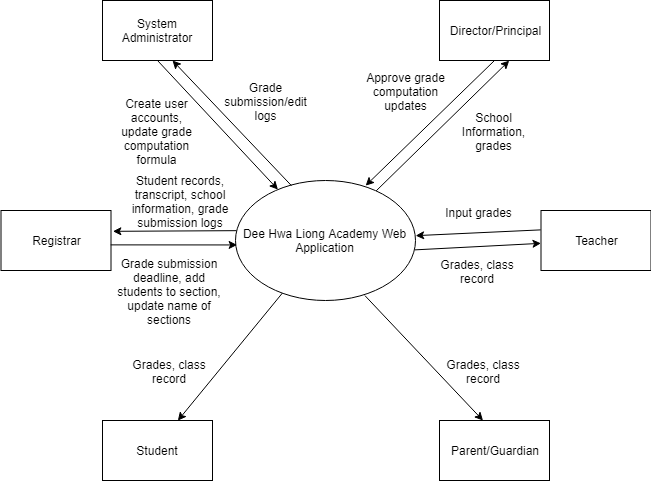
\includegraphics[height=10.5cm]{Context-Diagram.png}
\end{center}
\vspace{2cm}
\begin{center}
    Figure 1 - Context Diagram, Students' Grade Management System
\end{center}

\newpage
\subsection{Activity Diagrams}

All accounts will have a login and logout function. Each user account can also change the account's password. The password change is done within the system. No external links will be provided for password change. Profiles for each account will be available and can be updated.

The system administrator is the one managing the system.

The user can create accounts for the other users such as director, registrar, teachers, and students. All account creation will not have any creation requests.

The administrator is the only one with access to the activity logs of the condensed grade sheet. The activity log records every information changes that occur to grade sheets in the system. This activity log cannot be edited nor deleted, it is only readable. The administrator can also search the log using date, time, teacher's name, section, school year, grade level, and/or grade sheet name.

Activation and deactivation of accounts is also a functionality of the administrator. An account can be deactivated if the user is no long affiliated with the school.

Since DepEd may issue a change in the grading process of schools, updating grade computation formula is also included in the function of the administrator. Such changes can only occur if the school director approves these changes.

As mentioned earlier, some changes or updates can only occur if the director approves it.

The director is the one who directs and shapes the curriculum and the teaching process of a school.

This user will be the one in charge of approving changes for grade computation formula. Furthermore, he can also view grades of each subject and the condensed grades. Viewing of summary reports is also possible.

Summary reports will get all the information needed from the database of the system.

The school registrar is in charge of keeping student records.

The school registrar will be able to set the deadline for submission of grades. Different deadlines may be set for different teachers due to their workload differences. Deadline alerts will be automatically sent, by the system, during 5 days and 3 days before the deadline and during the deadline day.

Since a school registrar keeps student records, they can view record from past school years and produce TORs. Viewing of summary reports will also be possible. Summary reports may be requested by the principal, director, and/or the DepEd and PEAC.

School registrars can update the student list of each section by adding or removing students from the class list. They can also update the section name and view the submitted grade of teachers.

Another activity log will be present under this user, which is the submission logs of teachers. This will be used to check the teachers who failed to comply with the deadline set by the registrar.

A school will never be a school without its teachers. In this system, there are two types of teachers: teacher-only and teacher/advisers.

Both types can input and update the grades of students. Their grade sheets will be automatically be available after they input the class and subjects they are handling in their profiles.

Both teacher-only and advisers can also submit the grades through the application to create the condensed grades sheet. Before submitting the grades, the teacher must be sure that there are no errors with the record. A save function will be available to save changes made in the grade sheet.

The difference between teacher-only and teacher/adviser, teacher/adviser can view the condensed grades of their advisees from the profiles. In addition, teacher/adviser can view his/her advisees' report carrds after the condensed grades have been finalized.

Finally, the student, this user can only do simple things such as view grades from his/her past grade levels to present.

\vspace{2cm}
\begin{center}
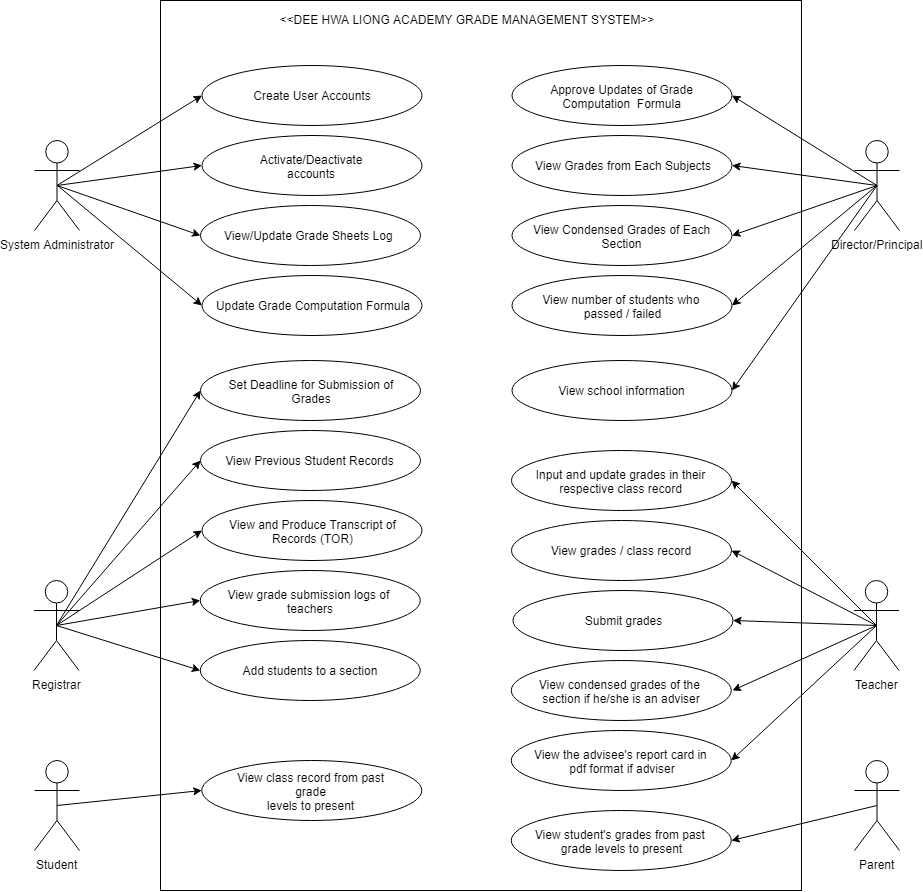
\includegraphics[height=14.5cm]{Activity-Diagram-1.png}
\end{center}
\vspace{2cm}
\begin{center}
    Figure 2 - Use Case Diagram, Students' Grade Management System
\end{center}

\newpage
\subsection{Database Design}

\subsubsection{Entity Relationship Diagram (ERD)}

Figure 1 shows the relationship among the user account, student, parent guardian, teacher, and nonacademic tables. The user account table contains the login credentials and basic information such as first name, last name, middle name, etc. of the user. System administrator, registrar, and principal/director fall under the nonacademic table.

Figure 2 shows the relationship among the grade sheet, category, grade, teacher, section, grade level, and subject. The grade sheet table contains the collection of grades of students in a section. The category table shows the type of activity being recorded in the grade sheet. The grade table contains an individual grade of the student, and other important information such as date, category, and entry number. The section table shows the section name of the class record. The subject table contains the subject code and the subject name of the grade sheet.

Figure 3 shows the relationship among the grade, student, category, and grade sheet. The grade table contains an individual grade of the student, and other important information such as date, category, and entry number. The category table shows the type of activity being recorded in the grade sheet. The grade sheet table contains the collection of grades of students in a section.

Figure 4 shows the relationship among the attendance log, teacher, and the student. The attendance log table contains the atendance information of a student in a specific day. The table also contains the studentID of the student and the teacher recording the attendance. 

Figure 5 shows the relationship among the advisory table, grade level, teacher and section. The advisory table contains the section being handled by the adviser. It also contains other information such as the grade level of the students being handled, the section, school year, and academic term. The teacher can only have an exact one advisory section. 

Figure 6 shows the relationship among the formula table, category, and grade level. The formula table shows the percentage of each component from each subject category per grade level. The category table shows the type of activity being recorded in the grade sheet. 

Figure 7 shows the relationship among the teacher load, subject, teacher, and section. The teacher load table shows the subject being handled by the teachers. Teachers can have multiple load since they can teach multiple sections throughout the academic year. They can also teach multiple subjects.

Figure 8 shows the relationship among submission deadline and teacher. The submission deadline tables contains the deadline date for the submission of grades of the teacher set by the registrar. Teacher can only have exactly one submission deadline.

\vspace{1cm}
\newpage
\begin{center}
    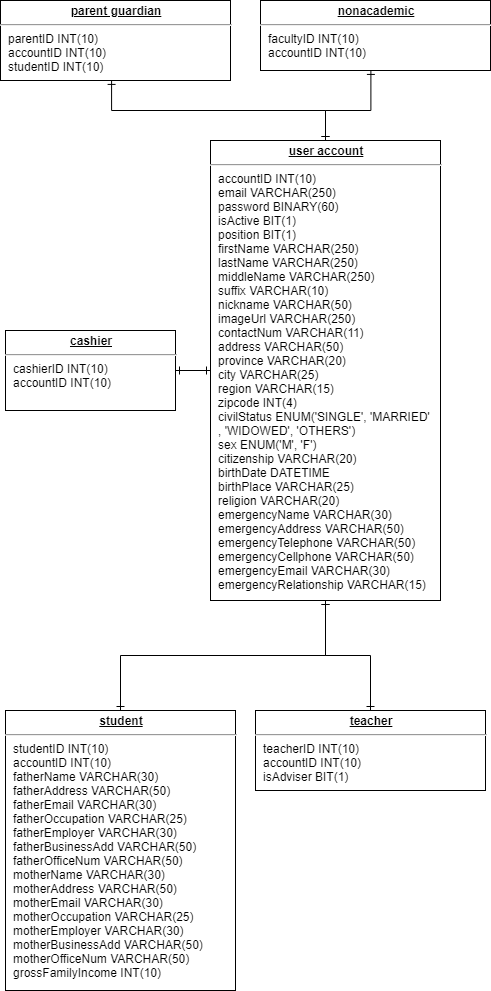
\includegraphics[height=19.5cm]{User.png}
\end{center}
\vspace{1cm}
\begin{center}
    Figure 1 - Entity Relationship Diagram (ERD) (user account)
\end{center}

\vspace{1cm}
\begin{center}
    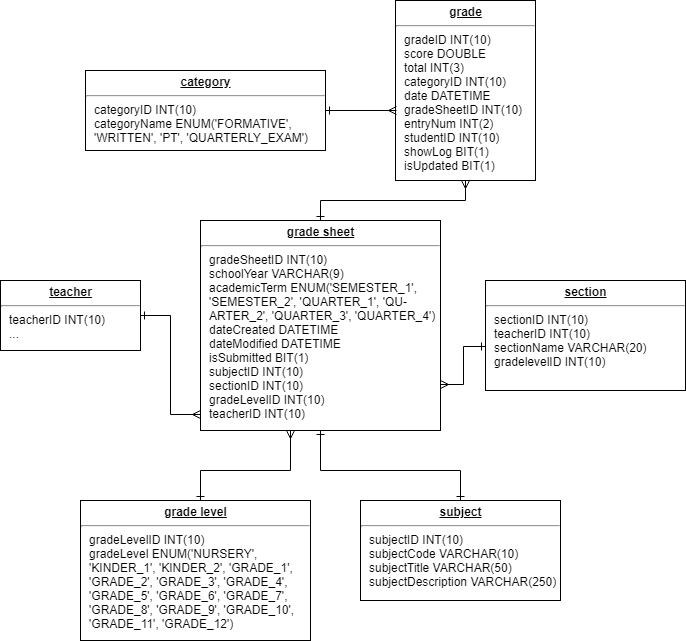
\includegraphics[height=13.5cm]{Grade-Sheet.png}
\end{center}
\vspace{1cm}
\begin{center}
    Figure 2 - Entity Relationship Diagram (ERD) (grade sheet)
\end{center}

\vspace{1cm}
\begin{center}
    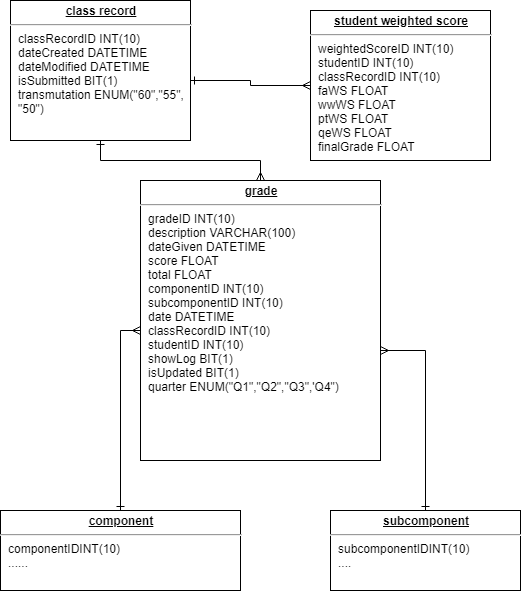
\includegraphics[height=8.5cm]{Grade.png}
\end{center}
\vspace{1cm}
\begin{center}
    Figure 3 - Entity Relationship Diagram (ERD) (grade)
\end{center}

\vspace{1cm}
\begin{center}
    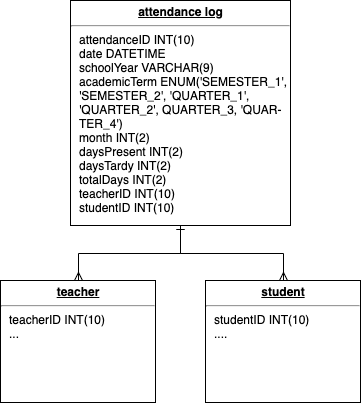
\includegraphics[height=8.5cm]{Attendance-Log.png}
\end{center}
\vspace{1cm}
\begin{center}
    Figure 4 - Entity Relationship Diagram (ERD) (attendance log)
\end{center}

\vspace{1cm}
\begin{center}
    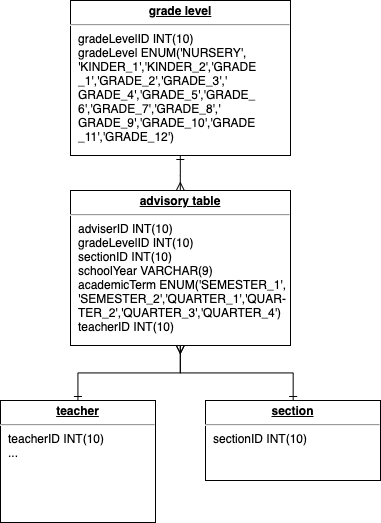
\includegraphics[height=10.5cm]{Advisory-Table.png}
\end{center}
\vspace{1cm}
\begin{center}
    Figure 5 - Entity Relationship Diagram (ERD) (advisory table)
\end{center}

\vspace{1cm}
\begin{center}
    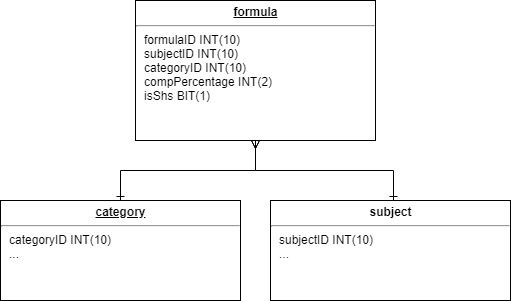
\includegraphics[height=8.0cm]{Formula.png}
\end{center}
\vspace{1cm}
\begin{center}
    Figure 6 - Entity Relationship Diagram (ERD) (formula)
\end{center}

\vspace{1cm}
\begin{center}
    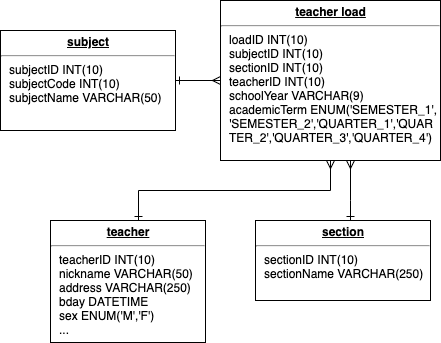
\includegraphics[height=6.5cm]{Teacher-Load.png}
\end{center}
\vspace{1cm}
\begin{center}
    Figure 7 - Entity Relationship Diagram (ERD) (teacher load)
\end{center}

\vspace{1cm}
\begin{center}
    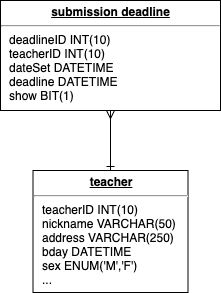
\includegraphics[height=6.5cm]{Submission-Deadline.png}
\end{center}
\vspace{1cm}
\begin{center}
    Figure 8 - Entity Relationship Diagram (ERD) (submission deadline)
\end{center}


\newpage

\subsection{Data Dictionary}

Shown below are the database tables. Primary keys are in bold format.

\subsubsection{User Account}

This table will provide the information needed to login.

\vspace{1cm}
\begin{longtable}{ |p{2.5cm}|p{4.5cm}|p{2.5cm}|p{3cm}|  }
    \hline
    \multicolumn{4}{|c|}{\textbf{user account}} \\
    \hline
    \textbf{FIELD}&\textbf{TYPE}&\textbf{KEY TYPE}&\textbf{DESCRIPTION}\\
    \hline
    \textbf{accountID}   & \textbf{INT(10), AUTO\_INCREMENT}   & \textbf{PRIMARY} & \textbf{Unique identifier of user}\\ \hline
    email & VARCHAR(250) & & Unique email address of user\\ \hline
    password & BINARY(60) & & Password of user in the system \\ \hline
    isActive & BIT(1) & & Denotes if the account is activated (1) or not (0)\\ \hline
    position & BIT(1) & & Denotes the account type: administrator (0), director (1), registrar (2), teacher (3), student (4), parent (5)\\ \hline
    firstName & VARCHAR(250) & & First name of the user \\ \hline
    lastName & VARCHAR(250) & & Last name of the user \\ \hline
    middleName & VARCHAR(250) & & Middle name of the user \\ \hline
    suffix & VARCHAR(10) & & Suffix of the user \\ \hline
    nickname & VARCHAR(50) & & Nickname of the user \\ \hline
    imageUrl & VARCHAR(250) & & Path to the photo of the user \\ \hline
    contactNum & VARCHAR(11) & & User's contact number \\ \hline
    address & VARCHAR(50) & & User's address \\ \hline
    province & VARCHAR(20) & & User's province \\ \hline
    city & VARCHAR(25) & & User's city \\ \hline
    region & VARCHAR(15) & & User's region \\ \hline
    zipcode & VARCHAR(4) & & User's zip code \\ \hline
    civilStatus & ENUM(`SINGLE', `MARRIED', `WIDOWED', `OTHERS') & & User's civil status \\ \hline
    sex & ENUM(`M', `F') & & User's sex \\ \hline
    citizenship & VARCHAR(20) & & User's citizenshipr \\ \hline
    birthDate & DATETIME & & User's birth date \\ \hline
    birthPlace & VARCHAR(25) & & User's birth place \\ \hline
    religion & VARCHAR(20) & & User's religion \\ \hline
    emergency- Name & VARCHAR(30) & & Contact name of the student in case of emergency \\ \hline
    emergency- Address & VARCHAR(50) & & Contact address of the student in case of emergency \\ \hline
    emergency- Telephone & VARCHAR(50) & & Telephone number of the student in case of emergency \\ \hline
    emergency- Cellphone & VARCHAR(50) & & Cellphone number of the student in case of emergency \\ \hline
    emergency- Email & VARCHAR(30) & & Contact email of the student in case of emergency \\ \hline
    emergency- Relationship & VARCHAR(15) & & Relationship of the student in the emergency contact \\ \hline
\end{longtable}

\vspace{1cm}
\begin{center}
Table 1: Data dictionary for \textbf{user account} table
\end{center}
\newpage
\subsubsection{Student}

The table will contain information about the student. The gathered information fields came from Dee Hwa Liong Academy's Student Application form.

\vspace{1cm}
\begin{longtable}{ |p{2.5cm}|p{4.5cm}|p{2.5cm}|p{3cm}|  }
    \hline
    \multicolumn{4}{|c|}{\textbf{student}} \\
    \hline
    \textbf{FIELD}&\textbf{TYPE}&\textbf{KEY TYPE}&\textbf{DESCRIPTION}\\
    \hline
    \textbf{studentID}   & \textbf{INT(10), AUTO\_INCREMENT}  & \textbf{PRIMARY} & \textbf{Unique identifier of student}\\ \hline
    accountID& INT(10) & FOREIGN & Unique identifier of user \\ \hline
    fatherName& VARCHAR(30) &  & Student's father's name \\ \hline
    fatherAdd- ress& VARCHAR(30) &  & Student's father's address \\ \hline
    fatherEmail& VARCHAR(30) &  & Student's father's email \\ \hline
    fatherOccu- pation& VARCHAR(30) &  & Student's father's occupation \\ \hline
    fatherEmplo- yer& VARCHAR(30) &  & Student's father's employer \\ \hline
    fatherBusi -nessAdd& VARCHAR(30) &  & Student's father's business address \\ \hline
    fatherOffice -Num& VARCHAR(30) &  & Student's father's office \\ \hline
    motherName& VARCHAR(30) &  & Student's mother's name \\ \hline
    motherAdd -ress& VARCHAR(30) &  & Student's mother's address \\ \hline
    motherEmail& VARCHAR(30) &  & Student's mother's email \\ \hline
    motherOccu- pation& VARCHAR(30) &  & Student's mother's occupation \\ \hline
    motherEmplo- yer& VARCHAR(30) &  & Student's mother's employer \\ \hline
    motherBusi -nessAdd& VARCHAR(30) &  & Student's mother's business address \\ \hline
    motherOffice -Num& VARCHAR(30) &  & Student's mother's office \\ \hline
\end{longtable}

\vspace{.5cm}
\begin{center}
    Table 2: Data dictionary for \textbf{student} table
\end{center}

\newpage

\subsubsection{Parent/Guardian}

The table will contain information about the parent/guardian.

\vspace{1cm}
\begin{longtable}{ |p{2.5cm}|p{4.5cm}|p{2.5cm}|p{3cm}|  }
    \hline
    \multicolumn{4}{|c|}{\textbf{parent guardian}} \\
    \hline
    \textbf{FIELD}&\textbf{TYPE}&\textbf{KEY TYPE}&\textbf{DESCRIPTION}\\
    \hline
    \textbf{parentID}   & \textbf{INT(10), AUTO\_INCREMENT}  & \textbf{PRIMARY} & \textbf{Unique identifier of parent/guardian}\\ \hline
    accountID& INT(10) & FOREIGN & Unique identifier of user \\ \hline
    studentID& INT(10) & FOREIGN & Unique identifier of the parent/guardian\\ \hline
\end{longtable}

\vspace{.5cm}
\begin{center}
    Table 3: Data dictionary for \textbf{parent guardian} table
\end{center}

\newpage

\subsubsection{Teacher}

The table will contain basic information about the teacher.

\vspace{1cm}
\begin{longtable}{ |p{2.5cm}|p{4.5cm}|p{2.5cm}|p{3cm}|  }
    \hline
    \multicolumn{4}{|c|}{\textbf{teacher}} \\
    \hline
    \textbf{FIELD}&\textbf{TYPE}&\textbf{KEY TYPE}&\textbf{DESCRIPTION}\\
    \hline
    \textbf{teacherID}   & \textbf{INT(10), AUTO\_INCREMENT}  & \textbf{PRIMARY} & \textbf{Unique identifier of teacher}\\ \hline
    accountID& INT(10) & FOREIGN & Unique identifier of user \\ \hline
    isAdviser& BIT(1) & & Denotes if the teacher has an advisory class (1) or not (0) \\ \hline
\end{longtable}

\vspace{.5cm}
\begin{center}
    Table 4: Data dictionary for \textbf{teacher} table
\end{center}

\newpage

\subsubsection{Nonacademic}

The table will contain basic information about the system administrator, director/principal, and registrar.

\vspace{1cm}
\begin{longtable}{ |p{2.5cm}|p{4.5cm}|p{2.5cm}|p{3cm}|  }
    \hline
    \multicolumn{4}{|c|}{\textbf{nonacademic}} \\
    \hline
    \textbf{FIELD}&\textbf{TYPE}&\textbf{KEY TYPE}&\textbf{DESCRIPTION}\\
    \hline
    \textbf{facultyID}   & \textbf{INT(10), AUTO\_INCREMENT}  & \textbf{PRIMARY} & \textbf{Unique identifier of nonacademic}\\ \hline
    accountID& INT(10) & FOREIGN & Unique identifier of user \\ \hline
\end{longtable}

\vspace{.5cm}
\begin{center}
    Table 5: Data dictionary for \textbf{nonacademic} table
\end{center}

\newpage

\subsubsection{Section}

This table will contain all the names of sections.

\vspace{1cm}
\begin{longtable}{ |p{2.5cm}|p{4.5cm}|p{2.5cm}|p{3cm}|  }
    \hline
    \multicolumn{4}{|c|}{\textbf{section}} \\
    \hline
    \textbf{FIELD}&\textbf{TYPE}&\textbf{KEY TYPE}&\textbf{DESCRIPTION}\\
    \hline
    \textbf{sectionID}   & \textbf{INT(10), AUTO\_INCREMENT} & \textbf{PRIMARY} & \textbf{Unique identifier of section}\\ \hline
    teacherID & INT(10) & FOREIGN & Unique identifer and denotes the adviser of the section \\ \hline
    sectionName & VARCHAR(20) & & Denotes the name of the section \\ \hline
    gradeLevelID & INT(10) & FOREIGN & Unique identifier of the grade level \\ \hline
\end{longtable}

\vspace{.5cm}
\begin{center}
    Table 6: Data dictionary for \textbf{section} table
\end{center}

\newpage

\subsubsection{Subject}

This table will contain all the subjects offered by Dee Hwa Liong Academy.

\vspace{1cm}
\begin{longtable}{ |p{2.5cm}|p{4.5cm}|p{2.5cm}|p{3cm}|  }
    \hline
    \multicolumn{4}{|c|}{\textbf{subject}} \\
    \hline
    \textbf{FIELD}&\textbf{TYPE}&\textbf{KEY TYPE}&\textbf{DESCRIPTION}\\
    \hline
    \textbf{subjectID}   & \textbf{INT(10), AUTO\_INCREMENT} & \textbf{PRIMARY} & \textbf{Unique identifier of a subject}\\ \hline
    subjectCode & VARCHAR(10) & & Subject code of the subject \\ \hline
    subjectTitle & VARCHAR(50) & & Title of the subject \\ \hline
    subjectDes- cription & VARCHAR(250) & & Desciption of the subject \\ \hline
\end{longtable}

\vspace{.5cm}
\begin{center}
    Table 7: Data dictionary for \textbf{subject} table
\end{center}

\newpage

\subsubsection{Grade Level}

Grade Level table will contain the grade levels under Dee Hwa Liong Academy.

\vspace{1cm}
\begin{longtable}{ |p{2.5cm}|p{4.5cm}|p{2.5cm}|p{3cm}|  }
    \hline
    \multicolumn{4}{|c|}{\textbf{grade level}} \\
    \hline
    \textbf{FIELD}&\textbf{TYPE}&\textbf{KEY TYPE}&\textbf{DESCRIPTION}\\
    \hline
    \textbf{gradeLevelID}   & \textbf{INT(10), AUTO\_INCREMENT} & \textbf{PRIMARY} & \textbf{Unique identifier of a grade level}\\ \hline
    gradeLevel & ENUM('NURSERY', 'KINDER\_1', 'KINDER\_2', 'GRADE\_1', 'GRADE\_2', 'GRADE\_3', 'GRADE\_4', 'GRADE\_5', 'GRADE\_6', 'GRADE\_7', 'GRADE\_8', 'GRADE\_9', 'GRADE\_10', 'GRADE\_11', 'GRADE\_12') & & Grade level of a student \\ \hline
\end{longtable}

\vspace{.5cm}
\begin{center}
    Table 8: Data dictionary for \textbf{grade level} table
\end{center}

\newpage

\subsubsection{Category}

Category table will tell us what type of activity (formative assessment-seatwork, formative assessment-assignments, written work-quizzes, written work-others, performance task-oral participation, etc.) is being recorded in the grade sheet

\vspace{1cm}
\begin{longtable}{ |p{2.5cm}|p{4.5cm}|p{2.5cm}|p{3cm}|  }
    \hline
    \multicolumn{4}{|c|}{\textbf{category}} \\
    \hline
    \textbf{FIELD}&\textbf{TYPE}&\textbf{KEY TYPE}&\textbf{DESCRIPTION}\\
    \hline
    \textbf{categoryID}  & \textbf{INT(10), AUTO\_INCREMENT} & \textbf{PRIMARY} & \textbf{Unique identifier of a category}\\ \hline
    categoryName & ENUM('FORMATIVE', 'WRITTEN', 'PT', 'QUARTERLY\_EXAM') & & Name of category \\ \hline
\end{longtable}

\vspace{.5cm}
\begin{center}
    Table 9: Data dictionary for \textbf{category} table
\end{center}

\newpage

\subsubsection{Subcategory}

Subcategory table is a subcomponent of a specific component (formative assessment-seatwork, formative assessment-assignments, written work-quizzes, written work-others, performance task-oral participation, etc.) being recorded in the grade sheet.

\vspace{1cm}
\begin{longtable}{ |p{2.5cm}|p{4.5cm}|p{2.5cm}|p{3cm}|  }
    \hline
    \multicolumn{4}{|c|}{\textbf{category}} \\
    \hline
    \textbf{FIELD}&\textbf{TYPE}&\textbf{KEY TYPE}&\textbf{DESCRIPTION}\\
    \hline
    \textbf{subCategID}  & \textbf{INT(10), AUTO\_INCREMENT} & \textbf{PRIMARY} & \textbf{Unique identifier of a subcategory}\\ \hline
    categoryName & VARCHAR(20) & & Name of subcategory \\ \hline
\end{longtable}

\vspace{.5cm}
\begin{center}
    Table 10: Data dictionary for \textbf{subcategory} table
\end{center}

\newpage

\subsubsection{Grade Sheet}

This will consist of the grades of the students from every activity to condensed grades.

\vspace{1cm}
\begin{longtable}{ |p{2.5cm}|p{4.5cm}|p{2.5cm}|p{3cm}|  }
    \hline
    \multicolumn{4}{|c|}{\textbf{grade sheet}} \\
    \hline
    \textbf{FIELD}&\textbf{TYPE}&\textbf{KEY TYPE}&\textbf{DESCRIPTION}\\
    \hline
    \textbf{gradeSheetID}  & \textbf{INT(10), AUTO\_INCREMENT} & \textbf{PRIMARY} & \textbf{Unique identifier of a grade sheet}\\ \hline
    schoolYear   & VARCHAR(9)   & & Academic year the student is currently enrolled in\\ \hline
    academicTerm   & ENUM('SEMESTER\_1', 'SEMESTER\_2', 'QUARTER\_1', 'QUARTER\_2', 'QUARTER\_3', 'QUARTER\_4') &  & Academic term of the grade\\ \hline
    dateCreated   & DATETIME   & & Date when the grade sheet was created\\ \hline
    dateModified  & DATETIME   & & Date when the grade sheet was modified\\ \hline
    isSubmitted   & BIT(1)   & & Denotes if the grade has been submitted for deliberation (1) or not (0)\\ \hline
    subjectID   & INT(10)   & FOREIGN & Unique identifier of a subject\\ \hline
    sectionID   & INT(10)   & FOREIGN & Unique identifier of a section\\ \hline
    gradeLevelID   & INT(10)   & FOREIGN & Unique identifier of a grade level\\ \hline
    teacherID   & INT(10)   & FOREIGN & Unique identifier of a teacher\\ \hline
\end{longtable}
    
\vspace{.5cm}
\begin{center}
    Table 11: Data dictionary for \textbf{grade sheet} table
\end{center}

\newpage

\subsubsection{Grade}

This represents a grade entry in a grade sheet.

\vspace{1cm}
\begin{longtable}{ |p{2.5cm}|p{4.5cm}|p{2.5cm}|p{3cm}|  }
    \hline
    \multicolumn{4}{|c|}{\textbf{grade}} \\
    \hline
    \textbf{FIELD}&\textbf{TYPE}&\textbf{KEY TYPE}&\textbf{DESCRIPTION}\\
    \hline
    \textbf{gradeID}  & \textbf{INT(10), AUTO\_INCREMENT} & \textbf{PRIMARY} & \textbf{Unique identifier of a grade}\\ \hline
    score   & DOUBLE   & & Student's score \\ \hline
    total   & INT(3)   & & The total number of items \\ \hline
    categoryID   & INT(10)   & FOREIGN & Unique identifier of a category \\ \hline
    subCategID   & INT(10)   & FOREIGN & Unique identifier of a subcategory \\ \hline
    date   & DATETIME   & & Date when the grade was created \\ \hline
    gradeSheetID   & INT(10)   & & Unique identifier of a grade sheet \\ \hline
    entryNum   & INT(1)   & & Denotes the entry number of the grade in the grade sheet \\ \hline
    studentID   & INT(10)   & FOREIGN & Unique identifier of a student \\ \hline
    showLog & BIT(1) & &  Denotes if the grade update will be show in the update log \\ \hline
    isUpdated & BIT(1) & & Denotes if the grade is the initial input (0) or not (1) \\ \hline
\end{longtable}
    
\vspace{.5cm}
\begin{center}
    Table 12: Data dictionary for \textbf{grade} table
\end{center}

\newpage

\subsubsection{Attendance Log}

This will hold the record of attendance of each student.

\vspace{1cm}
\begin{longtable}{ |p{2.5cm}|p{4.5cm}|p{2.5cm}|p{3cm}|  }
    \hline
    \multicolumn{4}{|c|}{\textbf{attendance log}} \\
    \hline
    \textbf{FIELD}&\textbf{TYPE}&\textbf{KEY TYPE}&\textbf{DESCRIPTION}\\
    \hline
    \textbf{attendanceID}  & \textbf{INT(10), AUTO\_INCREMENT} & \textbf{PRIMARY} & \textbf{Unique identifier of an attendance}\\ \hline
    date   & DATETIME   & & School date\\ \hline
    schoolYear   & VARCHAR(9)   & & School year of the attendance log\\ \hline
    academicTerm   & ENUM('SEMESTER\_1', 'SEMESTER\_2', 'QUARTER\_1', 'QUARTER\_2', 'QUARTER\_3', 'QUARTER\_4') &  & Academic term of the attendance log\\ \hline
    month   & INT(2) &  & Month of the attendance record\\ \hline
    daysPresent   & INT(2) &  & Number of days the student is present\\ \hline
    daysTardy   & INT(2) &  & Number of days the student is tardy\\ \hline
    totalDays   & INT(2) &  & Total number of school days in that month\\ \hline
    teacherID   & INT(10)   & FOREIGN & Unique identifier of a teacher\\ \hline
    studentID   & INT(10)   & FOREIGN & Unique identifier of a student\\ \hline
\end{longtable}

\vspace{.5cm}
\begin{center}
    Table 13: Data dictionary for \textbf{attendance log} table
\end{center}

\newpage

\subsubsection{Advisory Table}

This table will show the section being handled by the adviser.

\vspace{.5cm}
\begin{longtable}{ |p{2.5cm}|p{4.5cm}|p{2.5cm}|p{3cm}|  }
    \hline
    \multicolumn{4}{|c|}{\textbf{advisory table}} \\
    \hline
    \textbf{FIELD}&\textbf{TYPE}&\textbf{KEY TYPE}&\textbf{DESCRIPTION}\\
    \hline
    \textbf{adviserID}  & \textbf{INT(10), AUTO\_INCREMENT} & \textbf{PRIMARY} & \textbf{Unique identifier of an advisory table}\\ \hline
    gradeLevelID   & INT(10) & FOREIGN & Unique identifier of a grade   \\ \hline
    sectionID   & INT(10)   & FOREIGN & Gives the unique identifier of a section if the teacher is an adviser\\ \hline
    schoolYear   & VARCHAR(9)   & & School year of the advisory table\\ \hline
    academicTerm   & ENUM('SEMESTER\_1', 'SEMESTER\_2', 'QUARTER\_1', 'QUARTER\_2', 'QUARTER\_3', 'QUARTER\_4')   & & Academic term of the advisory table\\ \hline
    teacherID & INT(10) & FOREIGN & Unique identifier of a teacher\\ \hline
\end{longtable}

\vspace{.5cm}
\begin{center}
    Table 14: Data dictionary for \textbf{advisory table} table
\end{center}

\newpage

\subsubsection{Teacher's Load}

This table shows the subjects handled by different teachers.

\vspace{1cm}
\begin{longtable}{ |p{2.5cm}|p{4.5cm}|p{2.5cm}|p{3cm}|  }
    \hline
    \multicolumn{4}{|c|}{\textbf{teacher load}} \\
    \hline
    \textbf{FIELD}&\textbf{TYPE}&\textbf{KEY TYPE}&\textbf{DESCRIPTION}\\
    \hline
    \textbf{loadID}  & \textbf{INT(10), AUTO\_INCREMENT} & \textbf{PRIMARY} & \textbf{Unique identifier of the teacher's load}\\ \hline
    subjectID   & INT(10) & FOREIGN & Unique identifier of a subject\\ \hline
    sectionID   & INT(10) & FOREIGN & Unique identifier of a section\\ \hline
    teacherID   & INT(10) & FOREIGN & Unique identifier of a teacher\\ \hline
    schoolYear   & VARCHAR(9)   & & School year of the teacher's load\\ \hline
    academicTerm   & ENUM('SEMESTER\_1', 'SEMESTER\_2', 'QUARTER\_1', 'QUARTER\_2', 'QUARTER\_3', 'QUARTER\_4')   & & Academic term of the teacher's load\\ \hline
\end{longtable}

\vspace{.5cm}
\begin{center}
    Table 15: Data dictionary for \textbf{teacher load} table
\end{center}

\newpage

\subsubsection{Submission Deadline}

This table will contain the deadlines set by the registrar.

\vspace{1cm}
\begin{longtable}{ |p{2.5cm}|p{4.5cm}|p{2.5cm}|p{3cm}|  }
    \hline
    \multicolumn{4}{|c|}{\textbf{submission deadline}} \\
    \hline
    \textbf{FIELD}&\textbf{TYPE}&\textbf{KEY TYPE}&\textbf{DESCRIPTION}\\
    \hline
    \textbf{deadlineID}  & \textbf{INT(10), AUTO\_INCREMENT} & \textbf{PRIMARY} & \textbf{Unique identifier of the submission deadline}\\ \hline
    teacherID   & INT(10) & FOREIGN & Unique identifier of a teacher\\ \hline
    dateSet   & DATETIME &  & When the deadline was set\\ \hline
    deadline   & DATETIME &  & Deadline of submission of grades\\ \hline
    show   & BIT(1) &  & Denotes if the Registrar will display the deadline to teachers (0) or not (1)\\ \hline
\end{longtable}

\vspace{.5cm}
\begin{center}
    Table 16: Data dictionary for \textbf{submission deadline} table
\end{center}

\newpage

\subsubsection{Formula}

This table will contain the computation formula for each grade level approved by the director.

\vspace{1cm}
\begin{longtable}{ |p{2.5cm}|p{4.5cm}|p{2.5cm}|p{3cm}|  }
    \hline
    \multicolumn{4}{|c|}{\textbf{formula}} \\
    \hline
    \textbf{FIELD}&\textbf{TYPE}&\textbf{KEY TYPE}&\textbf{DESCRIPTION}\\
    \hline
    \textbf{formulaID}  & \textbf{INT(10), AUTO\_INCREMENT} & \textbf{PRIMARY} & \textbf{Unique identifier of the formula}\\ \hline
    sectionID & INT(10) & FOREIGN & Unique identifier of a section\\ \hline
    subjectID & INT(10) & FOREIGN & Unique identifier of a subject\\ \hline
    teacherID & INT(10) & FOREIGN & Unique identifier of a teacher\\ \hline
    subCategID & INT(10) & FOREIGN & Unique identifier of a subcategory\\ \hline
    categoryID & INT(10) & FOREIGN & Unique identifier of a category\\ \hline
    compWeight & INT(2) & & The weight of the component per subject category\\ \hline

\end{longtable}

\vspace{.5cm}
\begin{center}
    Table 17: Data dictionary for \textbf{formula} table
\end{center}

\newpage

\subsection{System Architecture}

Dee Hwa Liong Academy Web Application will be built under the Node.js server environment. Express.js will be used as a library for fetching data through API calls (using routers). The system will be using React.js library as the main front-end backbone. For the user interface, Ant Design, a design language made for React environment, alongside with Tabler React, an open-source UI framework for building dashboard applications will be used to make the website more responsive. MySQL will be used as the database of the system.

\subsection{Technical Architecture}

The students' grade management system will be accessed online. It follows a client-server-database architecture. The main server should have the following specifications (minimum requirements):

\vspace{1cm}

\textbf{System Technical Components}

\begin{enumerate}
    \item Node.js Run-time Environment for the Server (12.1.0 or higher)
    \item MySQL (7.2.10 or higher)
    \item Google Chrome (70.0.3538.102 or higher)
    \item Opera (56.0.3051.104 or higher)
    \item Microsoft Edge (42.17134.1.0 or higher)
    \item Internet Connection
\end{enumerate}






\section{Expected Output/Timeline}

\clearpage
\bibliographystyle{ieeetr}
\bibliography{biblio}

\end{document}


